% Standalone source of the figure fig:images: the image sources of the static fields at a welded interface.
% Build: pdflatex fig_images.tex; the paper includes the PDF. Grey scale only.
% z is depth and points down; interface z = 0; medium A above, medium B below.
% (a) Reflection: the force at x' in A, Kelvin's image x'* at the mirror point, and Mindlin's line of images on the
%     vertical half-line beyond x'* (uniform density for Phi1, density t - zeta for Phi2), seen from x in A.
% (b) Transmission: the potentials centred on x' itself, zeta = z - z', the line of images on the half-line
%     above x', seen from x in B.
\documentclass[border=2pt]{standalone}
% Shared preamble of the standalone figures of the interface paper.
\usepackage{amsmath,amssymb,bm}
\usepackage{tikz}
\usetikzlibrary{calc,arrows.meta}
\newcommand{\bR}{\mathbf{R}}
\newcommand{\bs}{\mathbf{s}}
\newcommand{\bu}{\mathbf{u}}
\newcommand{\bx}{\mathbf{x}}

\usetikzlibrary{decorations.pathreplacing}
\begin{document}
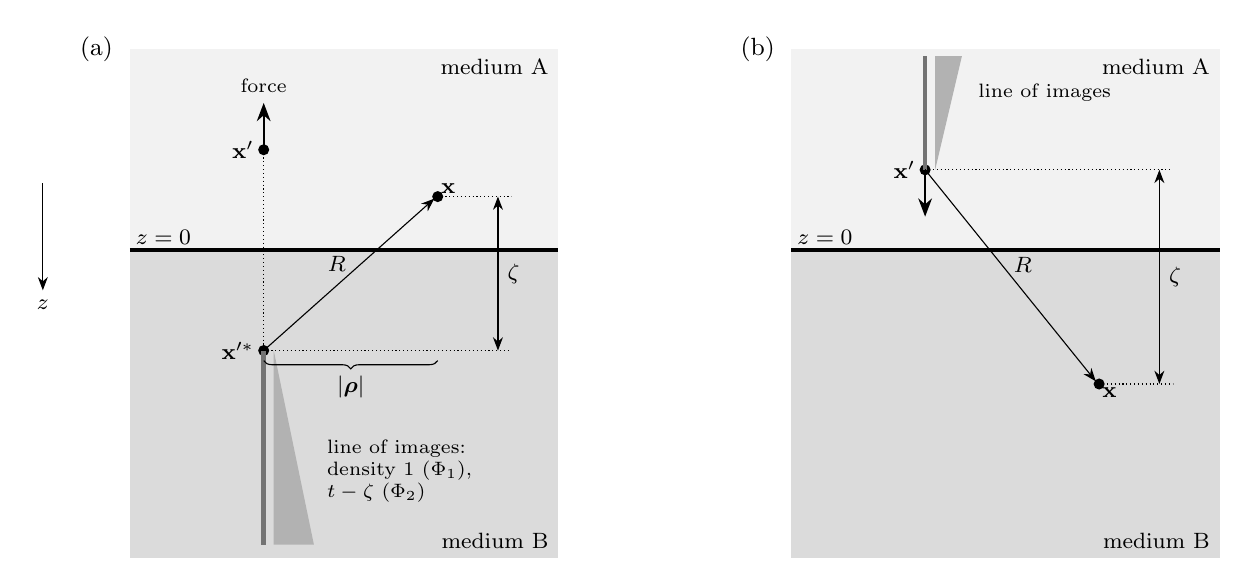
\begin{tikzpicture}[>=Stealth, x=0.85cm, y=0.85cm, font=\small]
  \newcommand{\media}[1]{%
    \fill[black!5] (-1.4,0) rectangle (5.0,3.0);
    \fill[black!14] (-1.4,-4.6) rectangle (5.0,0);
    \draw[very thick] (-1.4,0) -- (5.0,0);
    \node[anchor=north east, font=\footnotesize] at (5.0,3.0) {medium A};
    \node[anchor=south east, font=\footnotesize] at (5.0,-4.6) {medium B};
    \node[anchor=south west, font=\footnotesize, inner sep=2pt] at (-1.4,0) {$z=0$};
    \node at (-1.9,3.0) {#1};
  }
  % ---------------------------------------------------------------- (a) reflection
  \begin{scope}
    \media{(a)}
    % force and its image
    \fill (0.6,1.5) circle (2pt) node[left, font=\footnotesize] {$\mathbf x'$};
    \draw[->, thick] (0.6,1.5) -- (0.6,2.2) node[above, font=\scriptsize] {force};
    \fill (0.6,-1.5) circle (2pt) node[left, font=\footnotesize] {$\mathbf x'^{*}$};
    \draw[densely dotted] (0.6,1.5) -- (0.6,-1.5);
    % the line of images: uniform (Phi1) and growing (Phi2) densities
    \draw[line width=1.6pt, black!55] (0.6,-1.5) -- (0.6,-4.4);
    \fill[black!30] (0.75,-1.5) -- (0.75,-4.4) -- (1.35,-4.4) -- cycle;
    \node[anchor=west, font=\scriptsize, align=left] at (1.4,-3.3) {line of images:\\ density $1$ ($\Phi_1$),\\ $t-\zeta$ ($\Phi_2$)};
    % receiver, R and zeta
    \fill (3.2,0.8) circle (2pt) node[above right, font=\footnotesize, inner sep=1pt] {$\mathbf x$};
    \draw[->] (0.6,-1.5) -- (3.15,0.77) node[midway, above left, font=\footnotesize, inner sep=1pt] {$R$};
    \draw[densely dotted] (3.2,0.8) -- (4.3,0.8) (0.6,-1.5) -- (4.3,-1.5);
    \draw[<->] (4.1,0.8) -- (4.1,-1.5) node[midway, right, font=\footnotesize] {$\zeta$};
    \draw[decorate, decoration={brace, amplitude=3pt, mirror}] (0.6,-1.65) -- (3.2,-1.65)
      node[midway, below=2pt, font=\footnotesize] {$|\boldsymbol\rho|$};
  \end{scope}
  % ---------------------------------------------------------------- (b) transmission
  \begin{scope}[xshift=8.4cm]
    \media{(b)}
    \fill (0.6,1.2) circle (2pt) node[left, font=\footnotesize] {$\mathbf x'$};
    \draw[->, thick] (0.6,1.2) -- (0.6,0.5);
    % the line of images above the source
    \draw[line width=1.6pt, black!55] (0.6,1.2) -- (0.6,2.9);
    \fill[black!30] (0.75,1.2) -- (0.75,2.9) -- (1.15,2.9) -- cycle;
    \node[anchor=west, font=\scriptsize, align=left] at (1.25,2.35) {line of images};
    \fill (3.2,-2.0) circle (2pt) node[below right, font=\footnotesize, inner sep=1pt] {$\mathbf x$};
    \draw[->] (0.6,1.2) -- (3.15,-1.96) node[midway, above right, font=\footnotesize, inner sep=1pt] {$R$};
    \draw[densely dotted] (3.2,-2.0) -- (4.3,-2.0) (0.6,1.2) -- (4.3,1.2);
    \draw[<->] (4.1,1.2) -- (4.1,-2.0) node[midway, right, font=\footnotesize] {$\zeta$};
  \end{scope}
  \draw[->] (-2.7,1.0) -- (-2.7,-0.6) node[below, font=\footnotesize] {$z$};
\end{tikzpicture}
\end{document}
